%	PACKAGES AND OTHER DOCUMENT CONFIGURATIONS

\documentclass[11pt, a4paper]{article} % 10pt font size (11 and 12 also possible), A4 paper (letterpaper for US letter) and two column layout (remove for one column) Use additional titlepage argument to generate this
%\documentclass[12pt, a4paper,twocolumn,titlepage]{article}

%%%%%%%%%%%%%%%%%%%%%%%%%%%%%%%%%%%%%%%%%
% Wenneker Article
% Structure Specification File
% Version 1.0 (28/2/17)
%
% This file originates from:
% http://www.LaTeXTemplates.com
%
% Authors:
% Frits Wenneker
% Vel (vel@LaTeXTemplates.com)
%
% License:
% CC BY-NC-SA 3.0 (http://creativecommons.org/licenses/by-nc-sa/3.0/)
%
%%%%%%%%%%%%%%%%%%%%%%%%%%%%%%%%%%%%%%%%%

%----------------------------------------------------------------------------------------
%	PACKAGES AND OTHER DOCUMENT CONFIGURATIONS
%----------------------------------------------------------------------------------------

\usepackage[english]{babel} % English language hyphenation

\usepackage{microtype} % Better typography

\usepackage{verbatim} % Allows mulitline commenting

\usepackage{amsmath,amsfonts,amsthm} % Math packages for equations

\usepackage[svgnames]{xcolor} % Enabling colors by their 'svgnames'

\usepackage[hang, small, labelfont=bf, up, textfont=it]{caption} % Custom captions under/above tables and figures

\usepackage{subcaption}

\usepackage{booktabs} % Horizontal rules in tables

\usepackage{lastpage} % Used to determine the number of pages in the document (for "Page X of Total")

\usepackage{graphicx} % Required for adding images

\usepackage{enumitem} % Required for customising lists
\setlist{noitemsep} % Remove spacing between bullet/numbered list elements

\usepackage{sectsty} % Enables custom section titles
\allsectionsfont{\usefont{OT1}{phv}{b}{n}} % Change the font of all section commands (Helvetica)

\usepackage{siunitx}

%----------------------------------------------------------------------------------------
%	MARGINS AND SPACING
%----------------------------------------------------------------------------------------

\usepackage{geometry} % Required for adjusting page dimensions

\geometry{
	top=1cm, % Top margin
	bottom=1.5cm, % Bottom margin
	left=2cm, % Left margin
	right=2cm, % Right margin
	includehead, % Include space for a header
	includefoot, % Include space for a footer
	%showframe, % Uncomment to show how the type block is set on the page
}

\setlength{\columnsep}{7mm} % Column separation width

%----------------------------------------------------------------------------------------
%	FONTS
%----------------------------------------------------------------------------------------

\usepackage[T1]{fontenc} % Output font encoding for international characters
\usepackage[utf8]{inputenc} % Required for inputting international characters

\usepackage{XCharter} % Use the XCharter font

%----------------------------------------------------------------------------------------
%	HEADERS AND FOOTERS
%----------------------------------------------------------------------------------------

\usepackage{fancyhdr} % Needed to define custom headers/footers
\pagestyle{fancy} % Enables the custom headers/footers

\renewcommand{\headrulewidth}{0.0pt} % No header rule
\renewcommand{\footrulewidth}{0.4pt} % Thin footer rule

\renewcommand{\sectionmark}[1]{\markboth{#1}{}} % Removes the section number from the header when \leftmark is used

%\nouppercase\leftmark % Add this to one of the lines below if you want a section title in the header/footer

% Headers
\lhead{} % Left header
\chead{\textit{\thetitle}} % Center header - currently printing the article title
\rhead{} % Right header

% Footers
\lfoot{} % Left footer
\cfoot{} % Center footer
\rfoot{\footnotesize Page \thepage\ of \pageref{LastPage}} % Right footer, "Page 1 of 2"

\fancypagestyle{firstpage}{ % Page style for the first page with the title
	\fancyhf{}
	\renewcommand{\footrulewidth}{0pt} % Suppress footer rule
}

%----------------------------------------------------------------------------------------
%	TITLE SECTION
%----------------------------------------------------------------------------------------

\newcommand{\authorstyle}[1]{{\large\usefont{OT1}{phv}{b}{n}\color{NavyBlue}#1}} % Authors style (Helvetica)

\newcommand{\institution}[1]{{\footnotesize\usefont{OT1}{phv}{m}{sl}\color{Black}#1}} % Institutions style (Helvetica)

\usepackage{titling} % Allows custom title configuration

\newcommand{\HorRule}{\color{SteelBlue}\rule{\linewidth}{1pt}} % Defines the gold horizontal rule around the title

\pretitle{
	\vspace{-30pt} % Move the entire title section up
	\HorRule\vspace{10pt} % Horizontal rule before the title
	\fontsize{32}{36}\usefont{OT1}{phv}{b}{n}\selectfont % Helvetica
	\color{Navy} % Text colour for the title and author(s)
}

\posttitle{\par\vskip 15pt} % Whitespace under the title

\preauthor{} % Anything that will appear before \author is printed

\postauthor{ % Anything that will appear after \author is printed
	\vspace{10pt} % Space before the rule
	\par\HorRule % Horizontal rule after the title
	\vspace{20pt} % Space after the title section
}

%----------------------------------------------------------------------------------------
%	ABSTRACT
%----------------------------------------------------------------------------------------

\usepackage{lettrine} % Package to accentuate the first letter of the text (lettrine)
\usepackage{fix-cm}	% Fixes the height of the lettrine

\newcommand{\initial}[1]{ % Defines the command and style for the lettrine
	\lettrine[lines=3,findent=4pt,nindent=0pt]{% Lettrine takes up 3 lines, the text to the right of it is indented 4pt and further indenting of lines 2+ is stopped
		\color{NavyBlue}% Lettrine colour gold DarkGoldenRod
		{#1}% The letter
	}{}%
}

\usepackage{xstring} % Required for string manipulation

\newcommand{\lettrineabstract}[1]{
	\StrLeft{#1}{1}[\firstletter] % Capture the first letter of the abstract for the lettrine
	\initial{\firstletter}\textbf{\StrGobbleLeft{#1}{1}} % Print the abstract with the first letter as a lettrine and the rest in bold
}

%	BIBLIOGRAPHY

\usepackage[backend=biber,style=phys,natbib=true,doi=false]{biblatex} 
%Can equally use numeric citation style without extra phys packaging (but doesn't change capitalisation), or authoryear for alphabetical listing without the codes (resembles APA)

%\addbibresource{references.bib} % The filename of the bibliography

\usepackage[autostyle=true]{csquotes} % Required to generate language-dependent quotes in the bibliography

%    APPENDICES

\usepackage[title]{appendix} %in appendix


 % Specifies the document structure and loads requires packages
\graphicspath{{"/Users/kit gallagher/Documents/Research Review/Report/Figures"}}
\newcommand*{\subscript}[1]{\ensuremath{_\textrm{{\scriptsize #1}}}}

%	ARTICLE INFORMATION

\title{Simulating Liquid Crystals}

%\author{
	%\authorstyle{Christopher Gallagher}}
\author{\authorstyle{Candidate 8277T} 
	%\institution{University of Cambridge \\
	\institution{Supervisors: Prof Erika Eiser, Mr Jiaming Yu}}
% Example of a one line author/institution relationship
%\author{\newauthor{John Marston} \newinstitution{Universidad Nacional Autónoma de México, Mexico City, Mexico}}

\date{\today} % Add a date here if you would like one to appear underneath the title block, use \today for the current date, leave empty for no date
\usepackage[UKenglish]{babel}
\usepackage{tabularx}
%\renewcommand{\thefootnote}{\roman{footnote}}  %use roman lettering for footnotes instead
%\usepackage[backend=biber,doi=false]{biblatex}
\addbibresource{reportreferences.bib}
%\AtBeginBibliography{\small}

\usepackage{atbegshi}% http://ctan.org/pkg/atbegshi
\AtBeginDocument{\AtBeginShipoutNext{\AtBeginShipoutDiscard}} %gets rid of spurious first page
%----------------------------------------------------------------------------------------
\begin{document}
	
%Your project should contain the following statement on the first page of the project: Except where specific reference is made to the work of others, this work is original and has not been already submitted either wholly or in part to satisfy any degree requirement at this or any other university.	A link to your on-line notebook should also be added to the first page of your report before uploading the project.

\begin{titlepage}
    \begin{center}
    	%\thispagestyle{firstpage} % Apply the page style for the first page (no headers and footers)
    	\pagenumbering{gobble}
        \vspace*{1cm}
        \maketitle % Print the title
        
        
        \lettrineabstract{The specificity of DNA base-pair interactions gives considerable functional control in the design of anisotropic nano-particles, enabling the formation of a range of liquid crystal phases. Initial benchmarked tests confine the critical volume fraction of the nematic phase transition for linear ds-DNA mesogens (aspect ratio 10) to within $0.39<\phi<0.44$, in agreement with the theoretical value of $\phi = 0.4$.  I then introduce a novel `nunchuck' mesogen - two rigid rods of ds-DNA connected via a flexible linker of ss-DNA, and demonstrate the existence of an entropy\textendash driven phase transition to a quasi-nematic ($S_{n} = 0.58$) phase in this system. I outline further evidence for the existence of more exotic `herringbone', twisted-nematic and biaxial-nematic phases through the use of the pair-wise orientational correlation function. Finally, I present an alternative method for phase identification through the study of dynamic properties, and identify the formation of nematic and smectic phases through the measurement of directional diffusion coefficients.}
        
%        \begin{figure}[h!]
%        	\centering
%        	
\includegraphics[width=0.4\linewidth]{Figures/university-of-cambridge-seeklogo.com}
%        	\caption*{}
%        \end{figure}
        
        
        \vspace*{5cm}
        
        Supplementary Material: \textit{If necessary} \\
		Online Lab-book: \textit{To be included} \\
		
		\vspace*{2cm}
%		
		Except where specific reference is made to the work of others, this work is original and has not been already submitted either wholly or in part to satisfy any degree requirement at this or any other university.
        
       
        
    \end{center}
\end{titlepage}

% \thispagestyle{empty} % use if starting numbering after contents page

\pagenumbering{arabic} %starts page numbering
\tableofcontents %contents page
\newpage


%	ABSTRACT

%\lettrineabstract{The specificity of DNA base-pair interactions gives considerable functional control in the design of anisotropic nano-particles, enabling the formation of a range of liquid crystal phases. Initial benchmarked tests confine the critical volume fraction of the nematic phase transition for linear ds-DNA mesogens to within 5\% of the theoretical value over a range of aspect ratios. I then introduce a novel `nunchuck' mesogen \textendash two rigid rods of ds-DNA connected via a flexible linker of ss-DNA, and demonstrate the existence of an entropy-driven phase transition to a quasi-nematic (S = 0.58) phase in this system. I outline further evidence for the existence of more exotic `herringbone', twisted-nematic and biaxial-nematic phases through the use of the pair-wise orientational correlation function. Finally, I present an alternative method for phase identification through the study of dynamic properties, and identify the formation of nematic and smectic phases through the measurement of directional diffusion coefficients.}

%TELL A STORY THROUGHOUT! - MAKE THE ARC CLEAR

\section{Introduction}

Since Kirkwood's prediction of an entropy-driven ordering transition in the freezing of hard spheres \cite{Kirkwood1954}, entropy-driven phase transitions have been the subject of much attention \cite{Kerr1993,Frenkel1999}. Their relevance to colloidal systems is often underestimated, but gives rise to a range of diverse phase behaviour \cite{Adams1998, Anderson2002, Forsyth1978}. In particular, a wealth of (primarily experimental) studies exists on `bent-core' liquid crystals -- rigid rods with a central bend \cite{Takezoe2006, Etxebarria2008, Yang2018}.

These molecules have primarily been used for their polarity; however, here we consider a bent-core system with no polarity, which displays true entropy-driven phase transitions. We conduct molecular dynamics simulations on a course-grained model to study such transitions in a system of ‘nunchucks’, molecules consisting of two rigid rods of double-stranded (ds-) DNA, connected via a flexible linker of single-stranded (ss-) DNA. This linker allows the configuration to vary from fully stretched to folded. 

DNA is chosen for its availability through polymerase chain reactions, its exact design in terms of sequence and, thus, its reproducibly on the nanoscale. The techniques in phase simulation developed here are relevant to more complex DNA structures, such as those used in the development of liquid crystal behaviour in DNA origami \cite{Cha2015,Wang2018}, or in entropy-driven nano-structure self-assembly \cite{Barry2010, Lin2000}.

In Section \ref{sec:Background}, I outline the thermodynamic theory behind liquid crystals and phase transitions, before describing the previous experimental and simulation work in this area. Section \ref{sec:Methods} details the computational approach taken in both simulation and analysis, and outlines the coarse-grained model used. I then benchmark the techniques used against known results for a system of rigid rods in Section \ref{sec:RigidRodSims}, outlining simulations from both dilute and crystalline initial configurations (with subsequent contraction or expansion respectively). These approaches are then applied to the nunchuck system in Section \ref{sec:Nunchuck_Sim}, with two separate coarse-grained representations of the central bend in the nunchuck molecules (fixed angle or fixed bond rigidity). Finally, I also consider a novel approach to phase characterisation through dynamic properties in Section \ref{sec:Dynamics}, using the anisotropy of the coordinate diffusion coefficients to identify the onset of order in dynamic simulations.


\section{Background} \label{sec:Background}
\subsection{Liquid Crystals}
%Include known phases etc - de gennes textbook gives useful milestone references 

First identified as an intermediary phase between solids and liquids in 1888 by Friedrich Reinitzer \cite{Reinitzer1888}, the fundamental classes of liquid crystals were characterised in subsequent decades by Georges Friedel (among others) \cite{Friedel1922}. Research into the applications of liquid crystals only became widespread in the 1960s however, initiated by the seminal research of George William Gray \cite{Gray1962}, and culminating in Heilmeier's development of the first liquid crystal display \cite{Heilmeier1969, Heilmeier1968}. Later, in 1991, Pierre-Gilles de Gennes  received the Nobel Prize in physics ``\textit{for discovering that methods developed for studying order phenomena in simple systems can be generalized to more complex forms of matter, in particular to liquid crystals and polymers}'' \cite{DeGennes1992}.

In the most general sense, liquid crystals are states of matter displaying properties between those of conventional liquids and solid crystals. For this reason, they are also known as mesomorphic phases, with individual molecules referred to as mesogens, and these terms will be used interchangeably through this report. While solid crystals display long range periodic order in three dimensions (and isotropic liquids in none), liquid crystals have a degree of long range order in some (but not all) spatial dimensions. Three fundamental classes of liquid crystal have been identified \cite{DeGennes1993}:

\begin{itemize}
	\item \textbf{Nematic:} No positional order, but orientational order as molecules tend to point in the same direction.
	\item \textbf{Smectic:} One-dimensional positional order, so has the appearance of 2D liquid layers separated by a well-defined spacing.
	\item \textbf{Columnar:} Two-dimensional positional order, so has the appearance of an 2D array of liquid tubes.
\end{itemize}

%\footnotemark \ %removed from after molecules
%\footnotetext{It should be noted that only achiral molecules may form nematic phases; chiral molecules form an equivalent cholesteric (or `twisted-nematic') phase. This is particularly relevant to the consideration of DNA; a chiral molecule.}

\begin{figure} [!ht]
	\centering
	\includegraphics[width=0.9\linewidth]{Figures/lc_phases_self1.png}
	\caption{Representation of the nematic and smectic phases for rod-like mesogens, in comparison to an isotropic liquid and a crystalline solid. Note that phases are ordered from left to right in terms of increasing volume fraction. Orientational order develops in the nematic phase, while positional order develops in the smectic phase, and is extended to all axes in the crystalline phase. Here, $\boldsymbol{\hat{n}}$ denotes the system director, and $\boldsymbol{\hat{n}}_{i}$ the director of an individual molecule. }
	\label{fig:lcphasescropped}
\end{figure}


It should be noted that the higher-order phases (smectic and columnar) also display orientational order throughout the body. This characteristic is fundamental to the formation of liquid crystals, and almost all mesogenic molecules are, therefore, anisotropic \cite{Kato2007}. We will see later that the degree of anisotropy affects the stability of different phases. 

This anisotropy can take different forms. `Rod-like' molecules (where anisotropy takes the form of one elongated axis) are the oldest, and most common, form of liquid crystal. They favour the formation of nematic and smectic phases, as visualised in Figure \ref{fig:lcphasescropped}, and are the focus of this report. Disk shaped (discotic) molecules, discovered by Chandrasekhar in 1977 \cite{Chandrasekhar1977}, have one compressed axis, and favour the formation of other nematic or columnar phases. In 1987, Lam predicted the existence of a sub-class of `bowlic' molecules that break the up-down symmetry of discotic molecules \cite{LinLei1988}, and these were subsequently found experimentally \cite{Zimmermann1985, Malthete1985}.

Liquid crystals can also be categorised by the driving force behind their transition. Samples containing only one type of smaller molecule undergo thermally-driven phase transitions are called thermotropic liquid crystals. In contrast, larger molecules or colloids dispersed in a continuous solvent are classed as lyotropic; their phase transitions are driven by concentration \cite{DeGennes1993}. Here, I focus on lyotropic, entropy-driven phase transitions, where the mesogen (here DNA-nanocolloid) interactions are purely repulsive. This study represents a benchmark for designer-made, DNA-based systems.

Entropy-driven phase transitions are often seen as counter-intuitive, as they rely on an increase in microscopic disorder from an increase in visible order (an example is given in Section \ref{sec:OnsagerTheory}). Although such transition were once considered an abnormality, Frenkel notably commented that `\textit{...such phase transformations may not be interesting exceptions, but the rule!}' \cite{Frenkel1999}.

\subsection{Onsager Theory} \label{sec:OnsagerTheory}

Onsager predicted a simple model of lyotropic, entropy-driven phase transitions \cite{Onsager1949}. Rod-like particles are modelled as thin spherocylinders with length $L$ and diameter $D$, and an excluded volume preventing overlap. The interaction potentials between the particles are neglected, and only the configurational entropy of the system considered. Qualitatively, the confinement of rods parallel to a director $\Vec{n}$, such as in the nematic phase, leads to a decrease in rotational entropy, but an increase in translational entropy, allowing rods to move freely parallel to one another. At sufficiently high concentrations, the translational entropy dominates, and the system undergoes a phase transition from isotropic to nematic. 

The critical volume fraction at transition is approximately $4D/L$ (see Appendix \ref{sec:OnsagerAppendix}). Thus, the isotropic--nematic phase transition occurs at lower concentrations for mesogens with greater aspect ratio, and requires a minimum aspect ratio of $L/D = 4$ to take place. It is worth noting that this result is only valid in the limit of thin spherocylinders, as Onsager's derivation neglects Virial coeffecients $B_{n}$ beyond the second order in the expansion of free energy in powers of density \cite{Frenkel1987}, as discussed in Appendix \ref{sec:OnsagerAppendix}. Onsager's theory has since been validated with both computational \cite{Frenkel1987b, Frenkel1988b} and experimental \cite{Kubo1979,Oldenbourg1988,Fraden1993} results.

%penultimate sentence could go into appendix
% validation of Onsagers theory in https://doi-org.ezp.lib.cam.ac.uk/10.1021/ar9500224
% also backed up in simulation context at start of rigid rods section


\subsection{Order Parameter}
%smectic order given by frenkel https://pubs.acs.org/doi/pdf/10.1021/j100322a042
%can also use https://www.tandfonline.com/doi/full/10.1080/00268976.2018.1471231

The degree of order in a liquid crystal phase is characterised by an order parameter, chosen such that it is unity in the fully ordered phase and zero in the isotropic phase. An example can be seen in the magnetisation $\textbf{M}$ of a ferromagnet: when raised above a critical temperature, the magnetisation vanishes as the ferromagnet undergoes a phase transition. While the choice of order parameter for the nematic phase transition is less intuitive than this example, it relies on the formation of genuine long-range orientational order. We may therefore define the angle ($\theta$) between each molecule's axis and the system director, such that the nematic order parameter $S_{n}$ can be written as:

\begin{equation} \label{eq:order_param}
S_{n} = \left\langle P_{2}(\cos(\theta)) \right\rangle = \left\langle \frac{3}{2}\cos^{2}(\theta) - \frac{1}{2} \right\rangle 
\end{equation} where $P_{2}$ denotes the second Legendre polynomial \cite{DeGennes1993}. While $\langle \cos^{2}(\theta) \rangle$ would function alone as the order parameter, (\ref{eq:order_param}) confines $S_{n}$ to values between unity for a perfectly aligned system, and zero for a completely random system. Further information on the motivation behind this choice, and how it is implemented in our simulation, is given in Appendix \ref{sec:NematicOrderAppendix}.

Similarly, it is helpful to define a smectic order parameter $S_{s}$ to characterise the formation of one-dimensional, long-range positional order. We can expect a non-zero Fourier component of the normalised density along the director \cite{Polson1997} and, thus, can write:

\begin{equation}
S_{s} = \frac{1}{N} \left\lvert \sum_{j=1}^{N} \exp \left( {\frac{2\pi}{L}i\textbf{r}_{j} \cdot \boldsymbol{\hat{n}}} \right) \right\rvert
\end{equation} for layers of periodicity $L$ perpendicular to the nematic director $\boldsymbol{\hat{n}}$, and where $\textbf{r}_{j}$ denotes the centre of mass position of the $j$th molecule \cite{Dussi2018}.


\subsection{DNA as a Liquid Crystal} 
%zhao2019 is useful review and gives onsager theory
%nakata is beyond onsager theory
%wang2018 gives useful section on history
Lyotropic liquid-crystalline phases are very common in living systems, from cellular membranes to fibroblast structures \cite{Stewart1966, Rey2013}. In vitro, many biochemical molecules - such as cellulose, peptides, and protein assemblies - have also been shown to form liquid crystal states \cite{Zhao2019}. With respect to the mesogenic behaviour of DNA, Luzzati et al. first observed a columnar phase in a condensed DNA solution in 1959 (only 6 years after the discovery of the double-helix structure), and Robinson pioneered the development of the twisted-nematic phase in 1961 \cite{Luzzati1959, Robinson1961}. Subsequent work by Strzelecka et al. has demonstrated experimentally that DNA molecules can form precholestric, cholestric and smectic phases (in order of increasing concentration) though lyotropic phase transitions \cite{Strzelecka1988}. 

Returning to Onsager's theory, with the known dimensions of DNA we find that that the minimum base pair length required to obtain liquid crystalline phase behaviour is 24 base pairs \cite{Bolhuis1997}. However this limit has been broken experimentally by Nakata et al. \cite{Nakata2007, Zanchetta2008}, who suggest this is a result of monomer stacking through end-to-end adhesion to form the larger mesogens required.

These techniques may be applied to developing DNA origami, the process whereby complex nano-structures are constructed out of DNA molecules. Through a greater understanding of the phase behaviour of DNA nanoparticles, we may inform the design of more complex structures, and develop colloidal self-assembly processes. These techniques may have applications in biophysics, photonics, structural biology and synthetic biology \cite{Nummelin2018, Praetorius2017, Bathe2017}.


\subsection{Previous Simulation Work} \label{sec:PrevWork}
Computational work may be implemented over a broad spectrum of coarse-graining, a process whereby microscopic degrees of freedom are integrated over to reduce the computational costs of a simulation at the cost of lower model resolution. The base unit of the simulation may range from single atoms to large bulk molecules \cite{Inglfsson2013, Potoyan2012}. Atomistic models, such as CHARMM \cite{MacKerell1995} and AMBER \cite{SalomonFerrer2012}, offer a greater level of detail, but are limited by computational cost beyond small (>30 base pairs) models \cite{Cheatham2004}. In contrast, bead-spring polymer models (with up to 3000 base pairs per bead) may obtain bulk material properties at significantly lower computational expense \cite{Michieletto2016}.

Such models have been applied specifically to DNA nunchucks by Salamonczyk et al. \cite{Salamonczyk2016} to suggest the existence of smectic phases. However, such models are limited by the level of coarse-graining applied, as the artificial interaction potentials considered have no physical origin. This project builds on Salamonczyk's research, by applying a intra-molecular potential derived from single nucleotide simulations of the nunchuck molecule by Jiaming Yu (within the Eiser Group) using OxDNA, a lower-level coarse grained model that accurately represents the physical properties of ss- and ds-DNA \cite{OxDNA}.

My work is based on a coarse-grained model developed by Xing et al. \cite{Xing2019} to consider Y-shaped nanoparticles constructed from DNA, using LAMMPS software\cite{LAMMPS} to model dense systems of these nunchuck nanoparticles. This approach allows us to simulate larger systems of DNA-mesogens, and provides a better predictor of the experimental phase behaviour of such systems.

\section{Methods} \label{sec:Methods}
All molecular dynamics (MD) simulations presented here were completed in LAMMPS (Large-scale Atomic/Molecular Massively Parallel Simulator), a medium coarse-grained, MD code developed to replicate solid-state materials and soft-matter mesoscopic systems \cite{Plimpton1995, LAMMPS}.


\subsection{Simulation Molecules} \label{sec:SimMolecules}
Here, we are considering `nunchuck' molecules formed of two rigid rods connected by a flexible linker, as depicted in Figure \ref{fig:nunchuck_analogy}. As the interaction potential of an anisotropic particle is rather complex, it is computationally simpler to consider each molecule as a system of connected spheres, each with a separate isotropic interaction potential (detailed further in Section \ref{pair_potential}). This system is visualised in Figure \ref{fig:nunchuck_implementation}, for rigid arms of aspect ratio 7. 

The ss-DNA is represented by a further sphere in the centre of the molecule, coloured red to highlight its differing mechanical properties. It has a modified bond angle, so the molecule is bent around this element, and reduced bond rigidity so the particle may also stretch about this point. We also consider a simplified system of rigid rods with no modifications of the central atom, to verify the analysis methods against known results.

\begin{figure}[ht]
	\hfill  %NOT SURE ABOUT THIS!
	\begin{subfigure}{.4\textwidth}
		\centering
		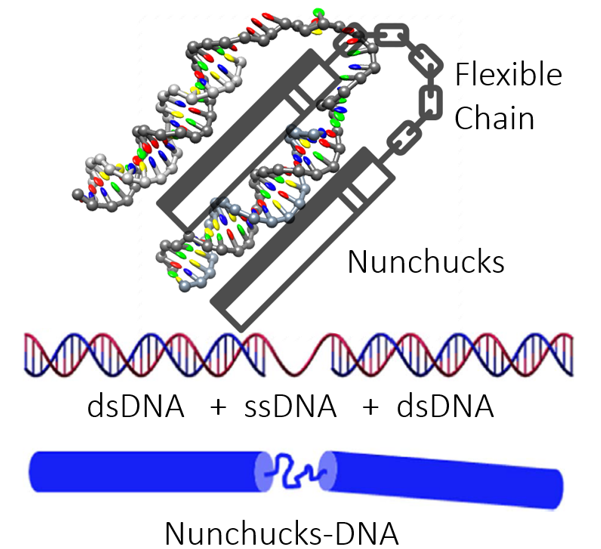
\includegraphics[width=\linewidth]{Figures/nunchucks_artist}  
		\caption{Coarse-grained Model}
		\label{fig:nunchuck_analogy}
	\end{subfigure}
	\hfill %% useful if width of each figure is less the .5\textwidth
	\begin{subfigure}{.4\textwidth}
		\centering
		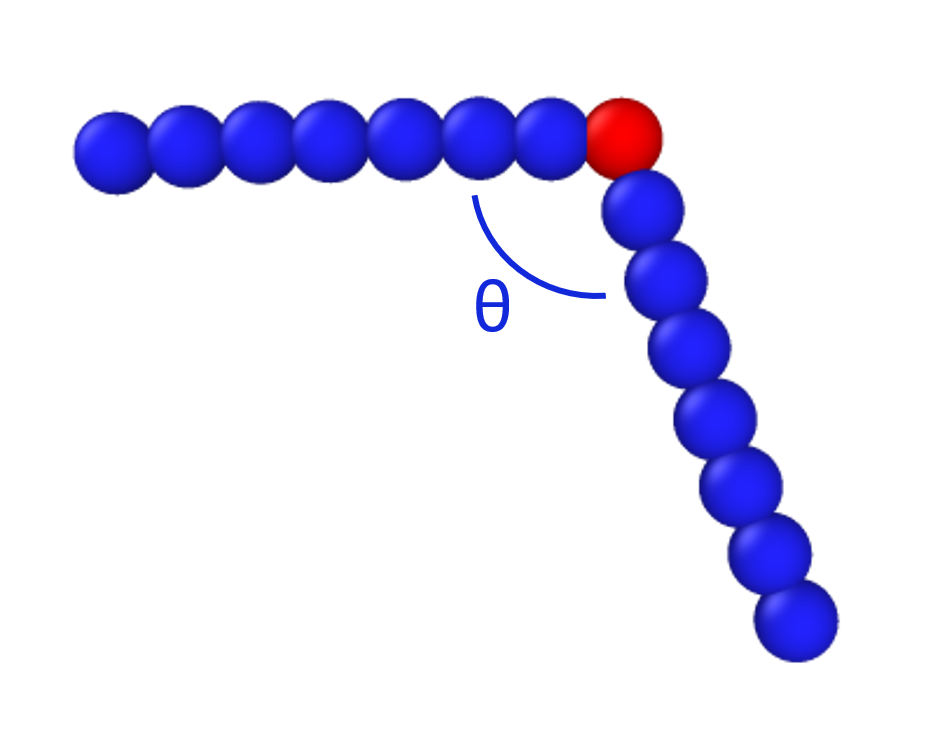
\includegraphics[width=\linewidth]{Figures/nunchuck_profile_coloured}  
		\caption{LAMMPS Implementation}
		\label{fig:nunchuck_implementation}
	\end{subfigure}
	\caption{Depiction of the analogy between the DNA mesogen and the nunchucks. Note the appearance of the flexible ss-DNA linker between the rigid ds-DNA rods, and the implementation within LAMMPS on the right. The central red sphere, representing the ss-DNA, is given modified bond properties to replicate the nunchuck's flexibility. Figure (a) created by Jiaming Yu (Eiser Group, Cambridge).}
	\label{fig:nunchucks_visual}
	\hfill
\end{figure}

A system of natural units was used in the simulations and replicated in our results here. Based on the Lennard-Jones potential, the cut-off length and characteristic energy were both set to unity. The simulation timescale was then fixed by the choice of these values and the mass of the simulation body. 

The physical values for a system may be considered for a specific system (in this case strands of ds-DNA) through scaling, via the relevant mass, length scale and energy scale of the system. However the dimensionless simulations presented here may be generalised to any similarly-shaped mesogens; we would expect other systems to display the same behaviour over an appropriate timescale determined by their material properties \cite{Rapaport2004}.

For the nunchuck particles considered, a length scale of \SI{2}{\nano\metre} was used (corresponding to the width of ds-DNA and hence the diameter of a simulation sphere) \cite{Arnott1972}. In comparison, the persistence length of DNA is around \SI{50}{\nano\metre} \cite{Garcia2007}, so the approximation of perfect rigidity is valid for all rods considered here (maximum length \SI{30}{\nano\metre}). Taking the average length of a base pair as \SI{0.33}{\nano\metre} \cite{Langridge1960}, each sphere corresponds to a sequence of six base pairs. This gives the mass of each sphere as \SI{6.5e-24}{\kilogram}, based on an average formula mass per base pair of \SI{650}{\dalton} \cite{Duewer2018}. 

From this, we may define the characteristic energy scale; this is formally the depth of the potential well in the full Lennard-Jones potential, but the thermal energy serves as a common approximation \cite{Pan2010} in agreement with experimental data \cite{Wang2002}. Using these values, we find that the characteristic timescale for this system is \SI{79}{\pico\second}. In this context, the simulation timestep would be \SI{0.4}{\pico\second}, and typical simulation of \num{20e6} steps had a total duration of \SI{7.9}{\micro\second}. For \num{1000} particles, this process took approximately $8$ hours to run on a standard laptop with an Intel Core i5 processor. %check these



\subsection{Simulation Structure} %was? is? check your tense here!
All simulations in this report were conducted on a system of 1000 particles, with a time step of $0.005\tau$, (where $\tau$ is the characteristic time), unless otherwise stated. The system was initially configured in a dilute, isotropic state; a non-trivial process for large numbers of mesogens as molecules must be placed randomly without overlap, to prevent any initial order affecting the subsequent formation of ordered phases. When studying high volume fractions, simulations were initiated from a perfectly ordered square crystalline phase, with all molecules aligned along a common axis. The choice of this axis is arbitrary, as the system is invariant under global rotation \cite{Nos1983}, but was taken to be directed along the $y$-axis for clarity. Care was taken to ensure molecules did not overlap, and that the system was stable in this ordered phase (i.e. internal energy was conserved over equilibration).

All simulations were conducted within an oblong box defined by the Cartesian axes, with periodic boundary conditions \cite{Frenkel2002}. The aspect ratio of this box may be varied, to support phase formation in anisotropic systems, as discussed in Section \ref{sec:PairWise_Application}. An isenthalpic ensemble (where pressure is fixed) was used to expand/contract the size of the simulation region, allowing sampling of different volume fractions from the same initial configuration. The microcanonical $(N,V,E)$ ensemble, with conserved volume and energy, was then used to allow the system to reach thermodynamic equilibrium. Time integration was evaluated using the Nos\'e\textendash Hoover thermostat \cite{Nos1984, Hoover1985} natively implemented in LAMMPS \cite{Shinoda2004}, with a damping time of $\tau$.

A typical simulation consists of multiple stages, alternating between these two ensembles to sample the system properties at a range of volume fractions. Approximately \num{2e4} steps were simulated when varying the simulation volume (depending on the resolution of volume fraction sampling), followed by \num{2e6} steps allowing the system to reach equilibrium in each stage. The output of thermodynamic variables, as well as particle positions, at the end of each stage allowed for the subsequent calculation of the order parameter at equilibrium. These data were retrieved at regular intervals during each simulation stage, to track the time evolution of the system.

To ensure the stability of the system, a Langevin thermostat \cite{Schneider1978} was used throughout, and energy conservation was verified over a range of timescales. The damping for all thermostats was equal to the characteristic timescale of the simulation (i.e. unity in natural units).



\subsection{Intermolecular Potential} \label{pair_potential}
A shifted, cut-off Lennard-Jones potential was chosen to represent pair-wise interactions between molecules. While the Lennard-Jones potential \cite{Jones1924a, Jones1924b} has long been the natural choice for molecular dynamics simulations \cite{Stephan2019}, its infinite range introduces computational complexity as interactions between all pairs of particles must be considered. It is therefore increasingly common to use a cut-off version, where the potential is set to zero beyond a `cut-off' radius; here, I chose to neglect the entire attractive tail. This simplified the calculations required, while also allowing our results to be generalised to any mesogens without attractive inter-molecular forces, that typically favour ordered-phase formation, as any phase transitions observed here must be purely entropy-driven. This is commonly known as a soft-core model, where particle overlap is suppressed via this repulsive potential rather than any excluded volume interactions, and is computationally much less demanding \cite{Paolini1993, Hughes2008}.

However, this cut-off may cause unphysical behaviour if the potential does not tend to zero smoothly. This is remedied by the addition of a constant term, described in the full form of the pair-wise potential $U_{ij}$:

\begin{equation} \label{lj_cut}
U_{ij} = 4\epsilon \left[ \left( \frac{\sigma}{r_{ij}} \right) ^{12} - \left( \frac{\sigma}{r_{ij}} \right) ^{6}	\right] + \epsilon \qquad	 r_{ij} < r_{c} = 2^{1/6} \sigma
\end{equation} Here $\sigma$ and $\epsilon$ are the relevant length and energy scales of the system, formally corresponding to the particle separation at which the $U_{ij} = 0$, and the depth of the potential well. It is worth noting that the effects of this truncation and shift on the overall thermodynamic quantities are well documented \cite{Stephan2020, Shaul2010}, and changes in lyotropic properties are negligible in 3D bulk liquids with a conserved particle number \cite{Smit1991}. This purely repulsive potential is also a good representation of the physical DNA system considered here, due to the effects of Debye screening \cite{Strey1997, Strey1998}.

 
\subsection{Analysis Methods}
We employed the visualisation freeware Ovito \cite{Ovito} to animate the mesogens motion and to generate all the particle images presented here. Thermodynamic variables, such as internal energy and pressure, were extracted to track the system's progress towards equilibrium and verify its stability.

The volume fraction and nematic order parameter were computed for comparison with Onsager's theorem, as detailed in Section \ref{sec:OnsagerTheory}. The calculation of the order parameter is complicated by the absence of an imposed director (i.e. if no electric field is applied), and I use the approach taken by Eppenga and Frenkel \cite{Eppenga1984} which is reproduced in Appendix \ref{sec:OrderParamCalc}.

Further analysis included the calculation of the smectic order parameter, and pair-wise orientational correlation coefficient, detailed in Section \ref{sec:PairWise_Application}. All scripts for data extraction and analysis were written by the candidate, and are attached as supplementary material.



\section{Rigid Rod Simulations} \label{sec:RigidRodSims}
%Used to benchmark sys etc and demonstrate techniques to identify phase transitions.
%Detail nematic phase transition (longrun4) and validation through onsager theory
%Extend this with the longer rods which continue to confirm this theory

First I studied a system of rigid rods to verify that the analysis methods used could reproduce Onsager's theory. We focused specifically on the isotropic-to-nematic phase transition, as it is well-studied and verified computationally through both Monte Carlo (MC) \cite{Frenkel1984, Lee1987} and MD simulations \cite{Allen1987, Camp1996}.

%not experimentally; long-range maier-snape is better here https://pubs.acs.org/doi/pdf/10.1021/j100303a008

\subsection{Shrinking the Simulation Box}

For rigid rods with an aspect ratio $L/D = 10$, Onsager's theory predicts a lyotropic phase transition at a critical volume fraction of $\phi  = 0.4$. Considering a system of \num{1000} rigid rods, formed of \num{10} sequentially connected `balls' (force-centres), I applied alternating stages of contraction (increasing the volume fraction) and equilibration steps (maintaining a constant volume). Each contraction stage consisted of between \num{1e4} and \num{5e4} steps (chosen to identify the critical volume fraction with maximal resolution, while verifying that the order parameter was approximately constant outside of this), while the equilibration stage ran for \num{2e6} steps. In this way, I was able to confine the possible critical volume fraction to the range $0.39 < \phi< 0.44$, as observed in Figure \ref{fig:rr_nemorderparam}, achieving good agreement with Onsager's prediction.

\begin{figure} [h!]
	\centering
	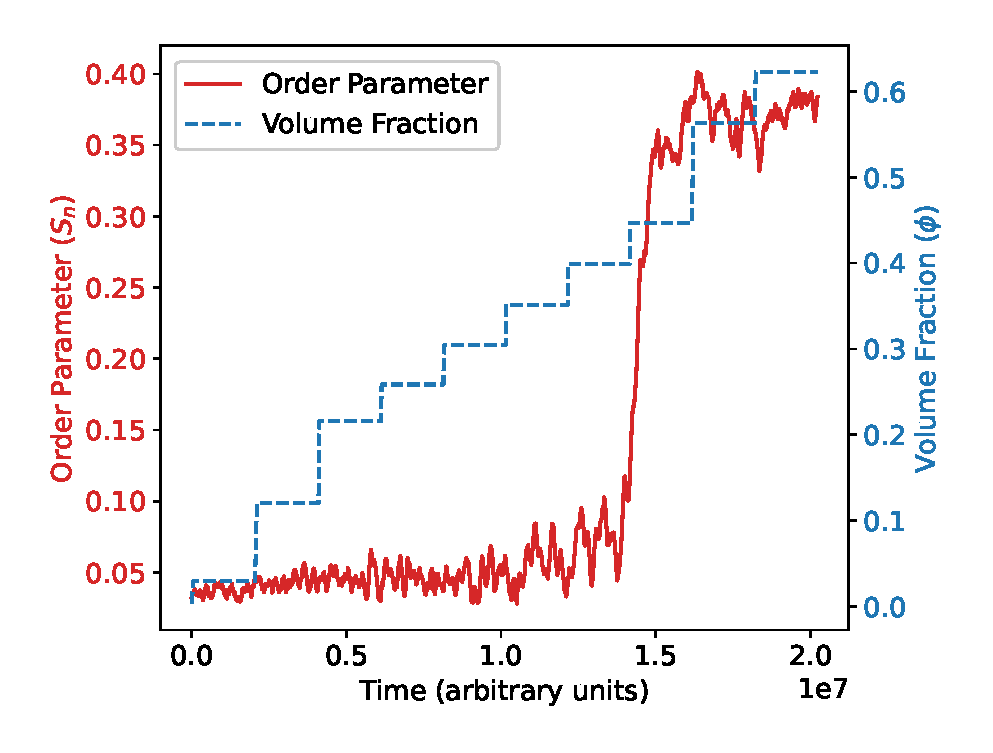
\includegraphics[width=0.7\linewidth]{Figures/rigidrod_nemorderparam}
	\caption{The evolution of the volume fraction and the nematic order parameter over the timescale of the simulation, for a system of 1000 rigid rods with aspect ratio 10. The jump in $S_n$ (red line) occurs at about $\phi \sim 0.4$. Note that the contraction steps, where the volume fraction is increased, are not of equal durations, and so do not correspond to equal changes in the system volume; rather they are chosen to highlight the phase transition. The contraction period is much shorter than the equilibration time, but the changes in volume fraction are not instantaneous, despite their appearance here.}
	\label{fig:rr_nemorderparam}
\end{figure}  %C:\Users\KitG\Documents\LC_Project\Phase_Structure\Rigid_Rods2

This analysis was repeated for longer rods with an aspect ratio of \num{16}, and a predicted critical volume fraction of $\phi  = 0.25$. My simulations verified that the critical volume fraction lies in the range $0.23 < \phi< 0.26$, in good agreement with the theory. This also provides a useful example of the characterisation of a phase transition through changes in the thermodynamic variables; Figure \ref{fig:rr_pressureevo} depicts a change in pressure during the equilibration stage, corresponding to the isotropic\textendash nematic phase transition.

\begin{figure} [h!]
	\centering
	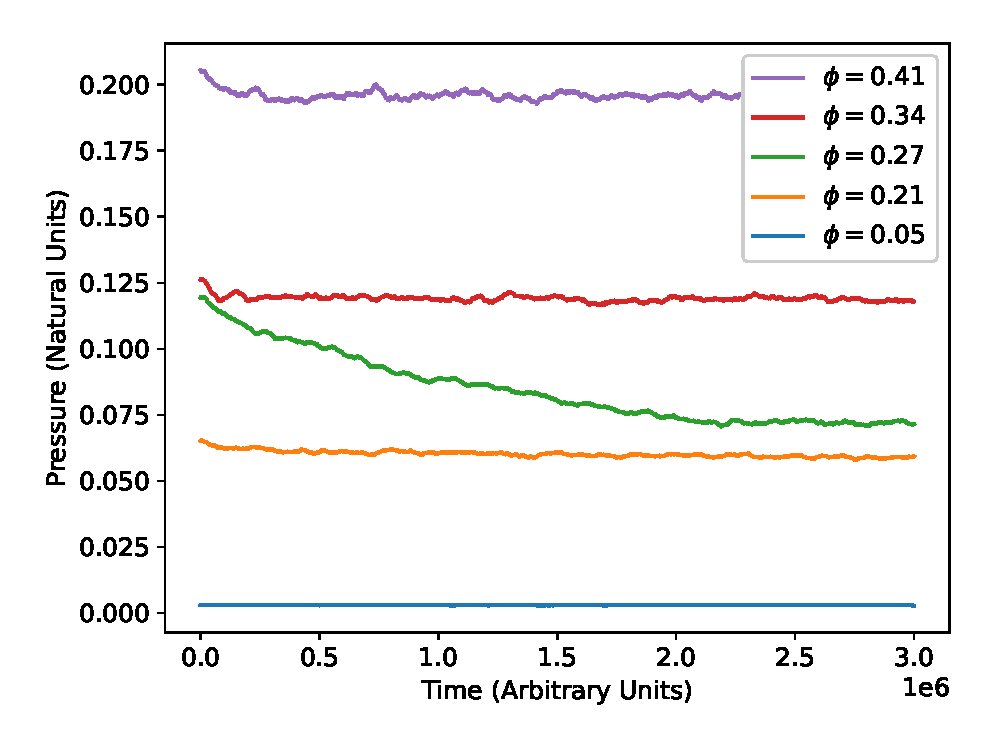
\includegraphics[width=0.7\linewidth]{Figures/rigidrod_pressureevo}
	\caption{The evolution of pressure on subsequent microcanonical ensembles (between which volume is decreased), when simulating 1000 rigid rods of aspect ratio 16. Note the extended decay in pressure for $\phi  = 0.27$, while the isotropic\textendash nematic phase transition occurs; all other stages remain at equilibrium throughout.}
	\label{fig:rr_pressureevo}
\end{figure} %C:\Users\KitG\Documents\LC_Project\Phase_Structure\Rigid_Rods2\Double_Length_Rods



\subsection{Expanding Simulations}
We also consider the phase behaviour upon expansion from a perfectly ordered state, in the hope of observing the same phase behaviour, as would be expected for an equilibrium system. This has two advantages: it allows us to access higher volume fractions that are not easily accessible through the shrinking procedure, and also provides verification of the phase transitions previously observed. Ensuring that a novel phase is in true equilibrium has long been a challenge for liquid crystal simulators; however, non-equilibrium effects will manifest themselves in a hysteresis of the phase transition (variation in the critical volume fraction dependent on the direction of the transition) and can, therefore, easily be identified through this method.

Initially, the particle force centres were placed on a simple cubic lattice. Again, equilibration was run in the microcanonical constant volume and alternated by an isenthalpic ensemble; however, the target pressure for the Nos\'e\textendash Hoover thermostat was reduced below the system pressure so that expansion occurred in these isenthalpic stages. The length of these stages remained unchanged from Section \ref{sec:RigidRodSims}; however, the thermostat damping was increased to $100\tau$ to ensure the stability of the expansion.

\begin{figure} [h!]
	\centering
	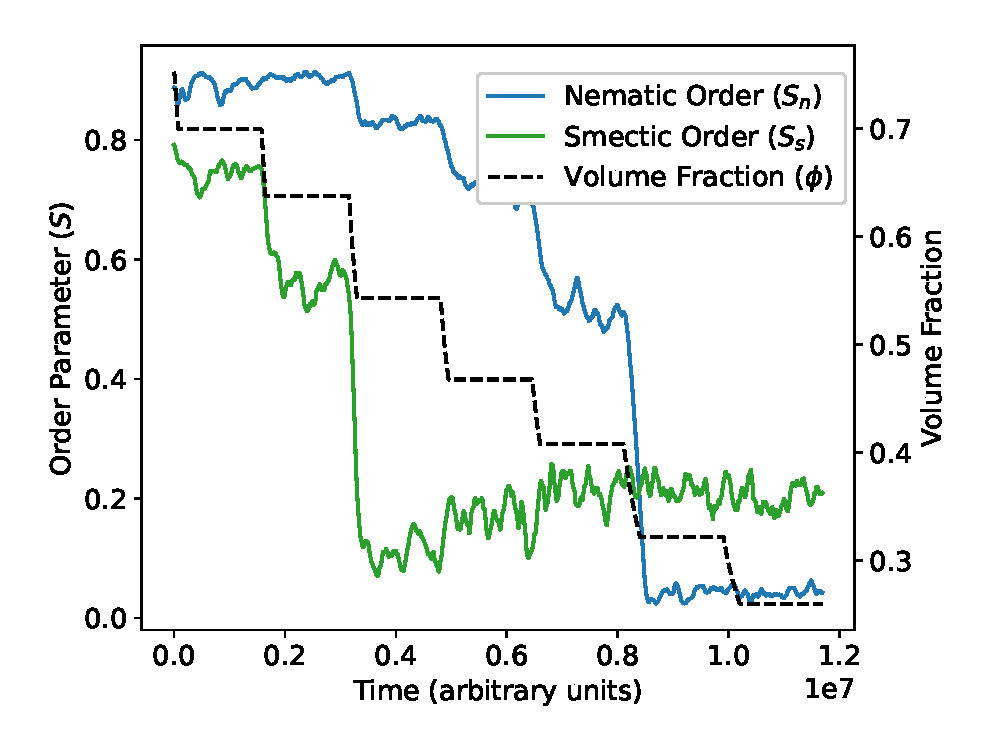
\includegraphics[width=0.7\linewidth]{Figures/rigidrod_cryorderparam}
	\caption{The evolution of the volume fraction against both the nematic ($S_{n}$) and smectic ($S_{s}$) order parameters over the timescale of the simulation, for a system of 1000 rigid rods with aspect ratio 10 initiated in a crystalline phase. A continuous smectic\textendash nematic phase transition is observed (in green) at high volume fractions, followed by a discrete nematic\textendash isotropic transition (in blue), occurring when $\phi$ is decreased below $0.4$. Note that there are multiple steps in the smectic order parameter, indicating this transition occurs over a range of volume fractions.}
	\label{fig:rr_crystalorder}
\end{figure} %C:\Users\KitG\Documents\LC_Project\Phase_Structure\Rigid_Rods2\Crystalline\Full_Transition


The isotropic phase formation was observed in the region $0.38 < \phi< 0.41$, in good agreement with the results of Section \ref{sec:RigidRodSims}, and confirming that this is indeed an equilibrium phase transition. 

The higher volume fractions accessed at the start of the simulation also gave rise to another phase transition, forming this nematic phase from the initial ordered phase. While the system was configured in a crystalline phase, it quickly relaxed into a smectic-like phase with one-dimensional long-range positional order. A subsequent smectic\textendash nematic transition was then observed with a reduction in the smectic order parameter around $\phi  = 0.6$, as shown in Figure \ref{fig:rr_crystalorder}. This transition is clearly concentration-dependent (with discrete jumps in the order parameter when the volume fraction is reduced); however, it occurs over a range of volume fractions and so was likely to be a continuous phase transition. While our evidence here is not conclusive, this is still a matter of active research and lies beyond the scope of this report. Theoretical \cite{Wen1987}, computational \cite{Frenkel1988, McGrother1996}, and experimental \cite{Dogic1997, Doane1972} evidence, however, suggests that this transition is expected to be continuous (or, at most weakly, first-order) for rigid rods of extended aspect ratios, and occurs around this volume fraction. 
%Frenkels results also find no dependance on aspect ratio (for crit volume frac)
%Later suggested that this transition is only continuous at large aspect ratios, and first order for ratios much smaller than are used here.
%Dogic suggests continuous for rigid particles, but first order if flexible, Doane uses hydrocarbon chains to come to the same conclusions

\section{Nunchuck Simulations} \label{sec:Nunchuck_Sim}
I applied the same simulation approaches to the nunchuck molecules introduced in Section \ref{sec:SimMolecules}. These could be configured in two ways: either with a fixed angle between the two rigid arms or with fixed rigidity (which determines the angular potential between the two arms, and hence the distribution of angles observed). Previous work by Jiaming Yu using OxDNA \cite{OxDNA} has suggested that the fixed rigidity model provides an accurate coarse-grained model of the DNA-nunchucks; however, the fixed-angle approach is also used for simplicity, and because it appears to be more amenable to ordered phase formation.


%different phases possible https://pubs.rsc.org/en/content/articlelanding/2011/SM/c1sm05751k#!divAbstract
%biaxial neamtics (feroomagnetic) https://pubs.acs.org/doi/pdf/10.1021/cm980631g
%dimers with central flexible spacer https://pubs.rsc.org/en/content/articlepdf/2014/tc/c4tc00212a

\subsection{Fixed Rigidity}
Initially, nunchucks with complete bond flexibility were considered. Despite this flexibility, a nematic-like phase was observed at volume fractions $\phi > 0.4$, with a maximal order parameter of \num{0.6} comparable to those measured previously in rigid rod systems. However, no uniform, system-wide director was observed, with the preferential orientation varying across the simulation region shown in Figure \ref{fig:nun_fr_views}.


\begin{figure}
	\centering
	\begin{subfigure}{.5\textwidth}
		\centering
		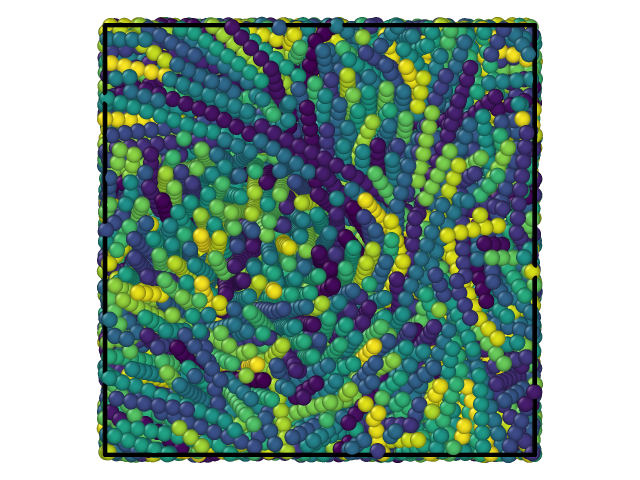
\includegraphics[width=.9\linewidth]{Figures/nun_fr_side}
		\caption{Side View}
		\label{fig:nun_fr_side}
	\end{subfigure}%
	\begin{subfigure}{.5\textwidth}
		\centering
		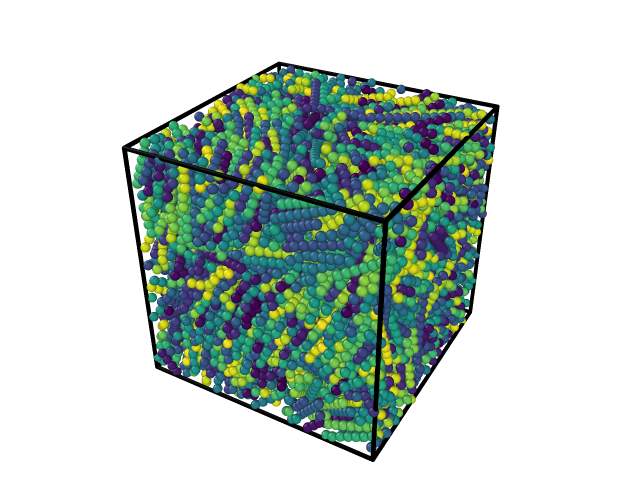
\includegraphics[width=.9\linewidth]{Figures/nun_fr_perspective}
		\caption{Perspective View}
		\label{fig:nun_fr_perspective}
	\end{subfigure}
	\caption{The quasi-ordered phase formed by \num{1000} fully flexible nunchucks. Note the local regions of aligned rods, suggesting a nematic-like phase, but also the variation of the director across the sample. The length scale of any periodicity in this variation is larger than the simulation box itself.}
	\label{fig:nun_fr_views}
\end{figure} %C:\Users\KitG\Documents\LC_Project\Phase_Structure\Nunchucks\Fixed_Rigidity\stretch500_rigidity5_len15

\begin{figure} [h!]
	\centering
	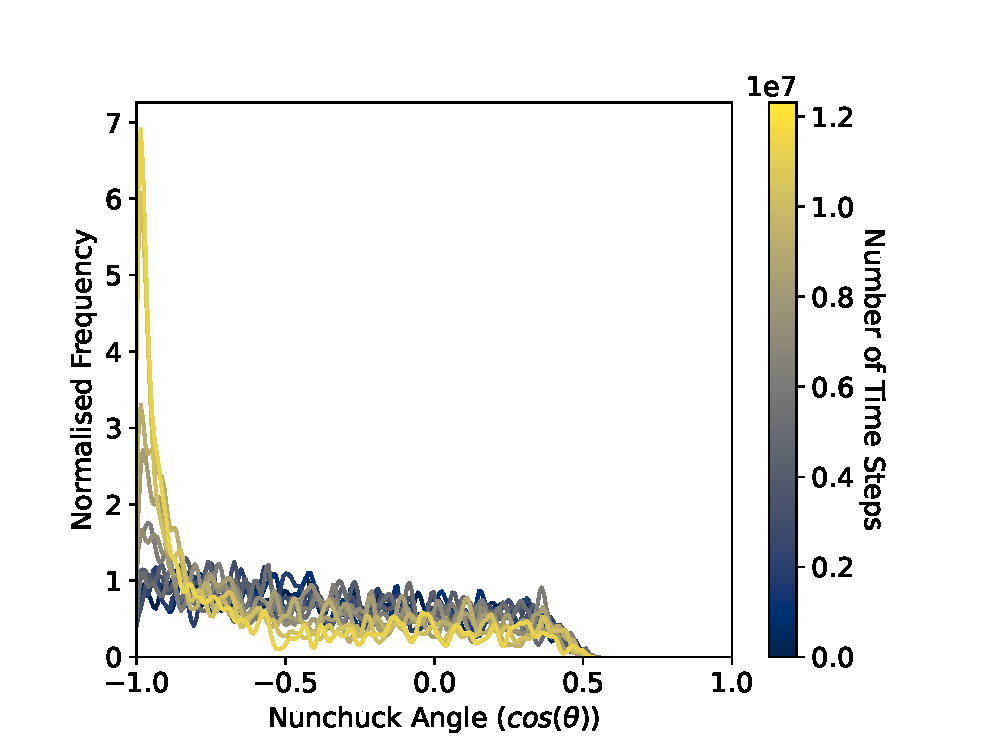
\includegraphics[width=0.7\linewidth]{Figures/nun_fr_angledist}
	\caption{A kernel density estimate plot of the distribution of nunchuck opening angle over time, as the volume fraction is reduced, for completely flexible nunchucks. Plotted for a system of \num{1000} particles, with the distribution sampled every \num{1e6} time steps. Note the formation of a preferential angle at late times, corresponding to the formation of an ordered phase at high volume fractions.}
	\label{fig:nun_fr_angledist}
\end{figure}  %C:\Users\KitG\Documents\LC_Project\Phase_Structure\Nunchucks\Fixed_Rigidity 

Consideration of the distribution of nunchuck bond angles (i.e. the opening angle between the two rigid arms) confirmed the formation of an ordered phase, with a clear preferential angle forming in Figure \ref{fig:nun_fr_angledist}. However, it is clear that any periodic variation of the director occurs on a length scale greater than the size of the simulation region, preventing further characterisation of this phase. Unfortunately the computational resources required to simulate larger systems exceeded those available in this research, due to the scaling of running time with particle number (which must increase to achieve the same density in larger volumes). 


\subsection{Fixed Angle}
I therefore considered systems where the nunchuck opening angle is confined to a particular value. I suggest that, in comparison to the fixed rigidity case, quasi-nematic structures may be observed on shorter length scales, particularly when the opening angle is confined below the mean angle (see Figure \ref{fig:nun_fr_angledist}).
I tested phase formation over a wide range of rigid rod lengths and opening angle values and broadly found that larger opening angles favoured nematic-like phase formation (with a maximal order parameter of $S_{n} = 0.62$), but smaller angles did not form obvious alternate ordered phases. Two such quasi-nematic phases are depicted in Figure \ref{fig:nun_fa_views}.

\begin{figure}
	\vspace{0.5cm}
	\centering
	\begin{subfigure}{.4\textwidth}
		\centering
		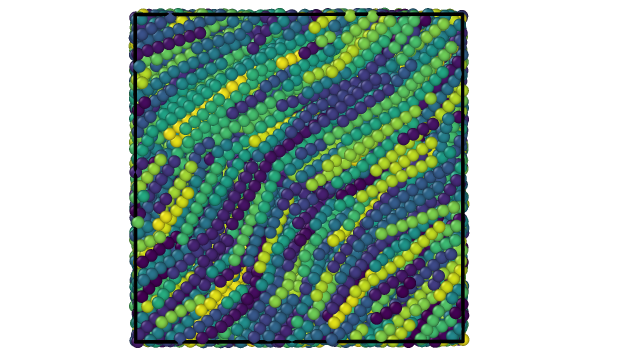
\includegraphics[width=.9\linewidth]{Figures/nun_fa_herringbone}
		\caption{Herringbone Structure}
		\label{fig:nun_fa_herringbone}
	\end{subfigure}%
	\begin{subfigure}{.6\textwidth}
		\centering
		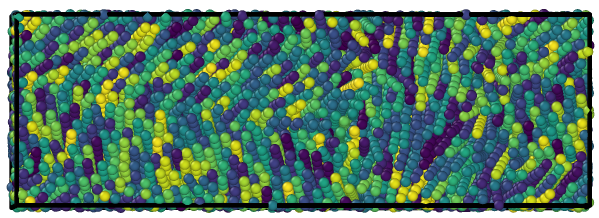
\includegraphics[width=.9\linewidth]{Figures/nun_fa_twist}
		\caption{Twisted Nematic Structure}
		\label{fig:nun_fa_twist}
	\end{subfigure}
	\caption{Two ordered phases formed separately by \num{1000} nunchucks with an opening angle of \ang{150}. Note the global alignment of molecule directors, giving a high nematic order parameter in either case. An alternating herringbone-like structure in observed in \textbf{(a)}, while the direction of the system director varies across the length of the simulation region in \textbf{(b)}, akin to a twisted nematic phase.}
	\label{fig:nun_fa_views}
\end{figure}

Alongside the tendency here to form a nematic phase with all molecules similarly aligned along a constant global director, there appears to be more periodic ordering, such as the herringbone structure clearly visible in Figure \ref{fig:nun_fa_herringbone}, or the rotation of the system director across the sample in Figure \ref{fig:nun_fa_twist} (typical of a twisted nematic phase). These structures cannot be described by our current order parameter methods.


\subsection{Orientational Order Parameter} \label{sec:PairWise_Application}
Alternative methods to characterise the order of the system are typically motivated by the class of symmetry expected. Given that our system appears to display a degree of orientational order, a length-dependent orientational order parameter is introduced to verify that this order is truly long-ranged and not simply due to short-range steric effects. This also allows the identification of any periodic aspects to the system as oscillatory components in the order parameter.

We consider an $l$-th rank, pair-wise correlation function, where $g_{l}(r)$ gives the correlation between the orientation of two particles separated by a distance $r$

\begin{equation} \label{eq:PairWise_eq}
g_{l}(r) = \frac{\langle P_{l}(\boldsymbol{\hat{u}_{i}}\cdot \boldsymbol{\hat{u}_{j}}) \delta(r_{ij}-r)\rangle}{\langle  \delta(r_{ij}-r) \rangle}
\end{equation} where $\boldsymbol{\hat{u}_{i}}$ is the director for molecule $i$, and $r_{ij}$ is the separation between a given pair of molecules $i$ and $j$ \cite{Zannoni1979}. In the disordered phase, this pair-correlation function decays to zero, while in the ordered phase it decays to the square of the orientational order parameter \cite{Frenkel1985b}:

\begin{equation}
\lim_{r \to \infty}g_{l}(r) = \left\langle P_{l} \right\rangle ^{2}
\end{equation}

Details of the simulation methods of $g_{l}(r)$ are given in Appendix \ref{sec:PairWise_Theory}. 

This may be applied to the systems shown in Figure \ref{fig:nun_fa_views}. However this approach is limited by the length scale of the simulation region; the maximum separation between particles is half the size of the simulation region due to the periodic boundary conditions \cite{Frenkel1985c}.

To determine order over longer length scales without increasing the volume of the system (due to limited computational resources), I instead varied the aspect ratio of the system. By considering an elongated oblong simulation region, such as in Figure \ref{fig:nun_fa_twist}, I was able to sample correlations over longer distances (along the long axis of the box) for systems of the same particle number. Using this method, the curves in Figure \ref{fig:num_fa_correlation_mol} confirm that the order observed in this fixed angle system is indeed long-range, with a non-decaying correlation at long length scales.

\begin{figure} [h!]
	\centering
	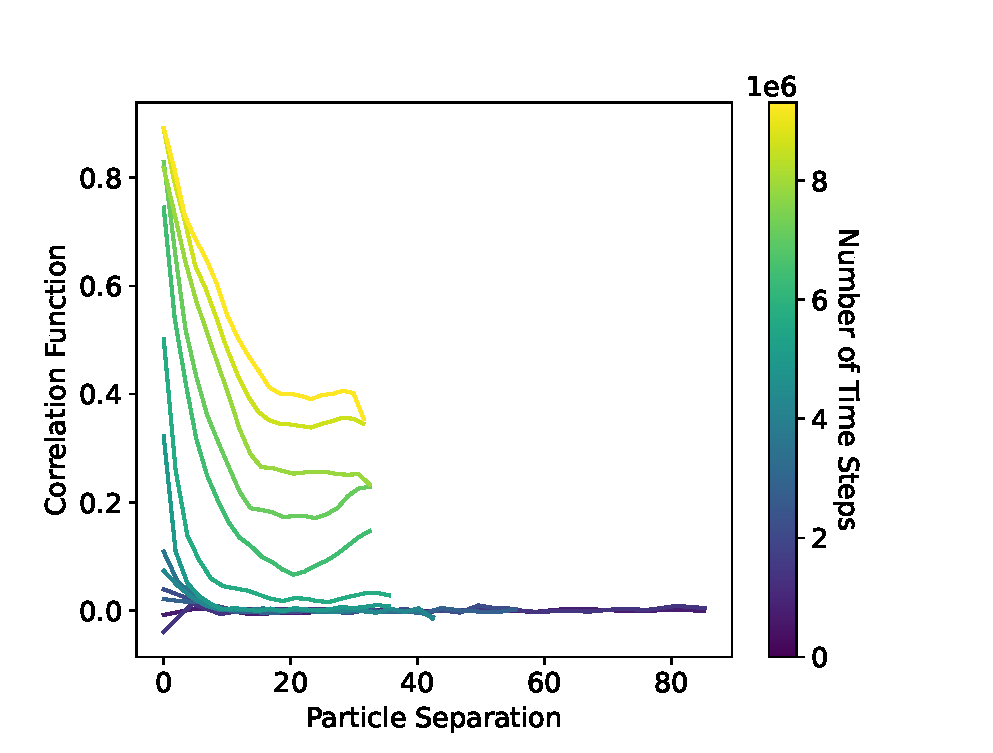
\includegraphics[width=0.7\linewidth]{Figures/num_fa_correlation_mol}
	\caption{Orientational correlation function over time (as the volume fraction is reduced), where nunchucks have a fixed opening angle. Plotted for a system of \num{1000} nunchuck molecules, with an opening angle of \SI{150}{\deg}, being sampled every \num{7e5} time steps. Note the formation of an ordered phase at high volume fractions (late times), with sustained long-range order (i.e. no decay in the orientational correlation function). The maximum value of particle separation (in arbitrary length units) is determined by the size of the simulation box, and so shrinks over time.}
	\label{fig:num_fa_correlation_mol}
\end{figure}  %C:\Users\KitG\Documents\LC_Project\Phase_Structure\Nunchucks\Fixed_Angle\2_bend_165_deg_oblong


This method is limited by the use of a single vector along the molecular axis to define the orientation of the molecule; two vectors are required to uniquely specify the orientation of a single nunchuck molecule. Using the molecular axis alone only accounts for quasi-nematic order and does not consider any biaxial or herringbone substructure. I therefore also considered additional orientational correlation functions for the bisector of each molecule, and normal vector to the plane of the nunchuck. The first Legendre polynomial is used to detect changes in sign of the bisector direction, as would be expected in a herringbone structure.

However, no statistically significant periodic components in the correlation function were observed over the length scale of the simulation region. A visual inspection of Figure \ref{fig:nun_fa_views} suggests that the length of the simulation region is approximately half the full period of the repeating structure, and so further research on larger simulation regions is required to verify these phases.


%LOOK INTO BIAXIAL\ SPLAY BEND NEMATIC PHASE FURTHER


\section{Dynamic Properties} \label{sec:Dynamics}
While the phase behaviour of rigid rods is well studied, much less is known about the dynamic properties of the individual mesogens within these quasi-ordered phases. This is, in part, due to the traditional popularity of MC approaches, which cannot predict dynamic properties. Nevertheless, dynamic studies through MD simulations have enjoyed recent popularity in both computational and experimental work \cite{GayBalmaz2013, Zhao2013, Rey2013}. Here, I undertake a brief study into the dynamic properties of the nunchuck system, and demonstrate the application of dynamic properties to static phase identification. In particular, I focus on the diffusion coefficient $D$ defined by the evolution of the mean-squared displacement (MSD) as a function of time $t$ in $n$ dimensions:

\begin{equation} \label{eq:msd_eq} 
\left\langle \left(x(t) - x_{0}\right)^{2} \right\rangle = 2nDt
\end{equation}

A derivation of this result is given in Appendix \ref{sec:Diffusion_Theory}. It is also instructive to consider the `power-law' formation of this relation \cite{Ernst2013}: 

\begin{equation}
\left\langle \left(x(t) - x_{0}\right)^{2} \right\rangle = 2nD_{\alpha}t^{\alpha}
\end{equation} which reduces to the pure-diffusive case of (\ref{eq:msd_eq}) when $\alpha=1$. Otherwise the process is characterised as subdiffusive ($\alpha < 1$) or superdiffusive ($\alpha > 1$) \cite{Metzler2000}. 

Displacements were only sampled over equilibration phases of our simulation, and the effect of the periodic boundary conditions was explicitly accounted for by offsetting additional displacements from boundary crossings. Linear regression analysis was used to predict the value of $\alpha$ for each run over a variety of volume fractions in the dilute limit. This limit occurs when each particle may exist in a non-overlapping free volume of rotation (a sphere circumscribed around the molecule), at a maximal volume fraction of

\begin{equation}
\phi_{dilute} = \frac{\pi(D/2)^{2}L}{\frac{4}{3}(L/2)^{3}} = \frac{3}{2} \left( \frac{D}{L}\right)^{2} 
\end{equation}

For rigid rods with an aspect ratio of 10, this gives a value of $\phi_{d} = 0.015$. We found an average power of $ \alpha = 0.97 \pm 0.03 $ for the nunchuck molecules, and $ \alpha = 1.00 \pm 0.04 $ for the rigid rods, as expected for diffusive behaviour. 

As the volume fraction was increased, I observed a tendency towards subdiffusive behaviour, with a reduction in the value of $\alpha$ to $0.12 \pm 0.02 $ at $\phi = 0.69$. This is given by the gradient when the root mean-squared (RMS) displacement is plotted over time in logarithmic space, as best demonstrated in Figure \ref{fig:nun_diff_rmsplots}, which depicts coordinate-wise displacement across three different phase regimes for a system of rigid rods. Here the Cartesian axes may be used, as simulations are configured in a crystalline phase with molecules orientated along the $y$ axis, and smectic layers forming in the $x-z$ plane. Phase transitions for this system have previously been identified in the regions $0.58<\phi<0.62$ for the smectic\textendash nematic, and $0.38<\phi<0.43$ for the nematic\textendash isotropic transition. 

At the highest volume fractions ($\phi \geq 0.62$), the diffusion along the $y$ axis is significantly reduced, due to the restricted motion between layers in the smectic phase. Below this, a nematic phase is observed with increased diffusivity along the molecule's director, corresponding to an increased intercept in logarithmic space. The degree of dynamic anisotropy here, quantified by the ratio of diffusion coefficients $D_{y}/D_{x}$, is $2.12$ for $\phi = 0.58$. At the lowest volume fractions ($\phi \leq 0.38$), there is no preferred direction in the system and motion is isotropic and truly diffusive (as $\alpha = 1$). 

\begin{figure} [h!]
	\centering
	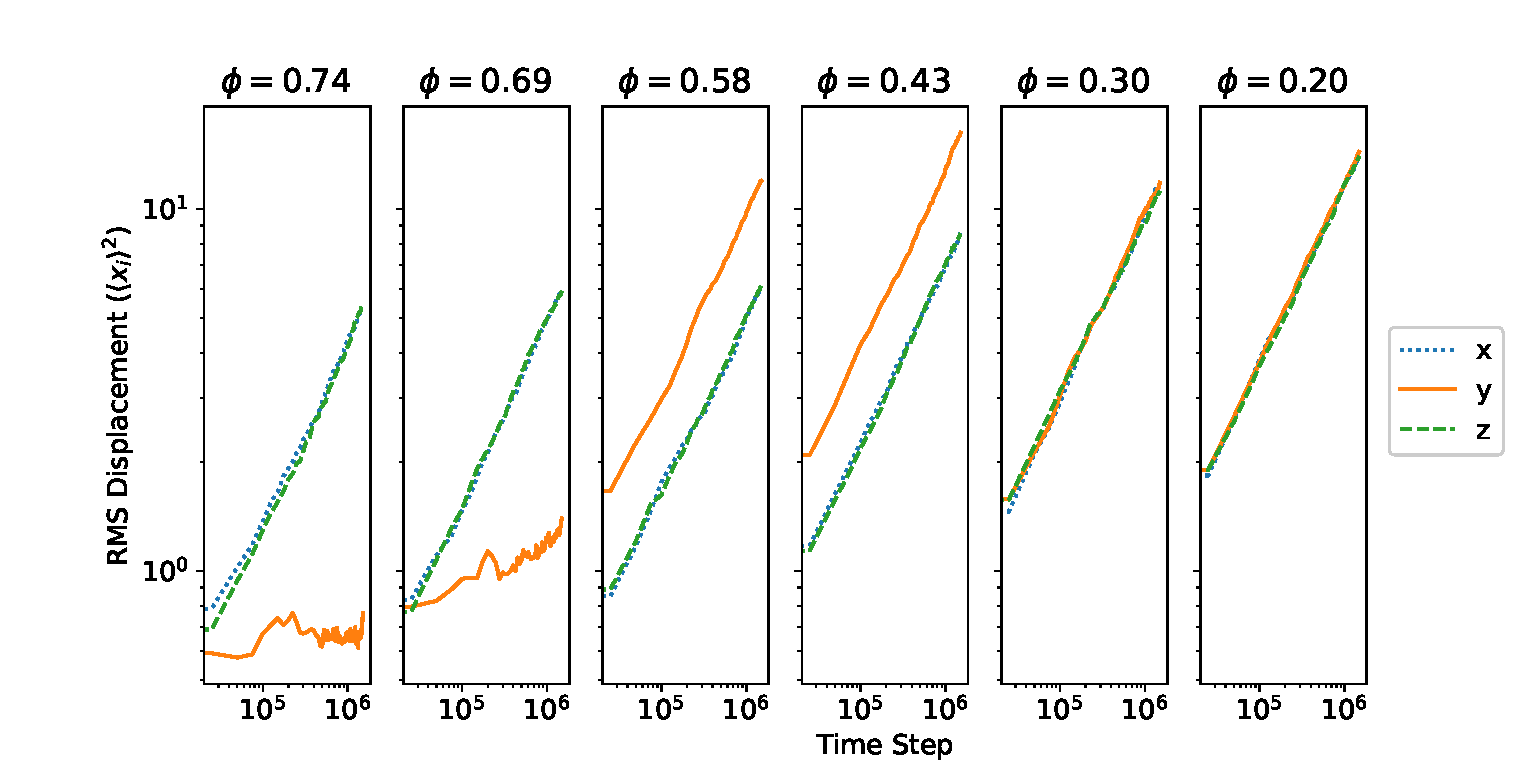
\includegraphics[width=\linewidth]{Figures/nun_diff_rmsplots}
	\caption{Root mean-squared displacements against time in a system of 1000 rigid rods with an aspect ratio 10, for a range of volume fractions $\phi$. The leftmost pair of plots correspond to the smectic phase, with restricted motion between $x-z$ layers along the $y$-axis. The centre pair give the nematic phase, with preferential displacement along the $y$-axis. Finally, the rightmost pair give the isotropic phase, with isotropic diffusion and no preferential direction. Note that no significant differences appear between the $x$- and $z$-directions in any phase, as these directions are equivalent in the phase structure.}
	\label{fig:nun_diff_rmsplots}
\end{figure}  %C:\Users\KitG\Documents\LC_Project\Phase_Structure\Rigid_Rods2\Crystalline\Full_Transition\Full_Transition2
Phase formation may also be observed through deviations in these coordinate-specific diffusion coefficients. Applying this analysis to the nunchuck system, isotropic diffusion is observed at low volume fractions in Figure \ref{fig:nun_diff_Dcoeff}. However, the $y$-coordinate diffusion coefficient is severely reduced beyond this, with an maximal anisotropy of $D_{y}/D_{x} = 0.19$ at $\phi = 0.58$. This strongly suggests the presence of a smectic phase below $\phi = 0.45$, in agreement with the prediction of $ 0.40<\phi<0.44$ obtained from the smectic order parameter. There is also some indication of the crystalline phase at the highest volume fractions, with diffusion equally limited in all directions, but this evidence is not conclusive.

\begin{figure} [h!]
	\centering
	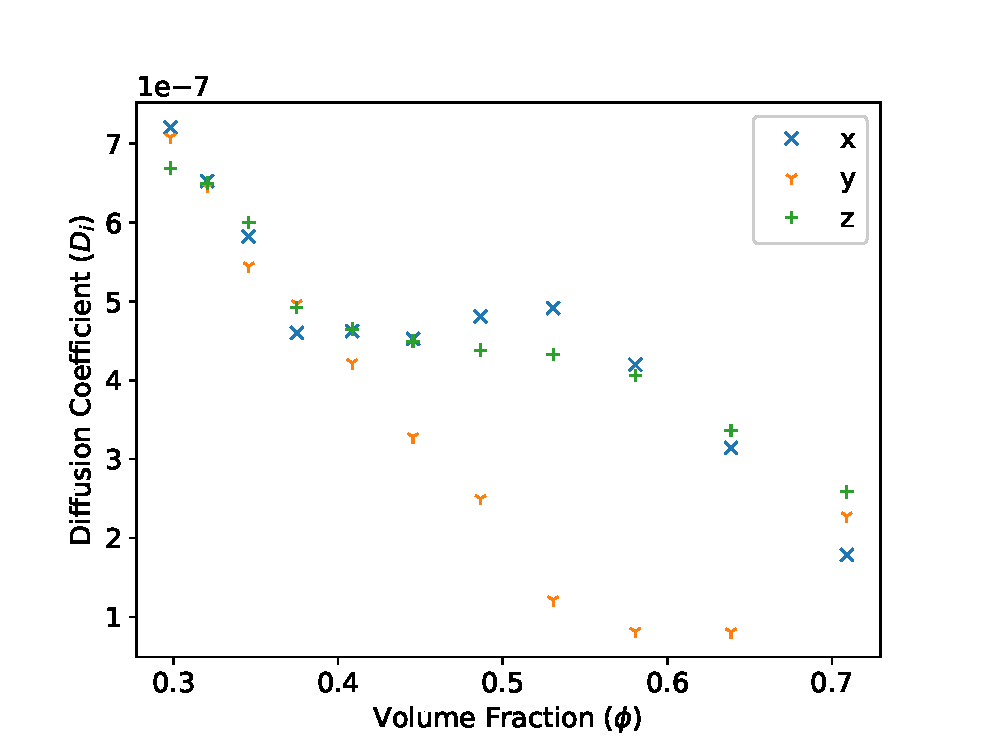
\includegraphics[width=0.7\linewidth]{Figures/nun_diff_Dcoeff}
	\caption{Coordinate diffusion coefficients for the evolution of the microcanonical ensemble under a range of volume fractions $\phi$. The low volume fraction region on the left of the graph corresponds to the isotropic phase, with no variation between coordinate axes. In contrast, the smectic phase in the high volume fraction gives rise to anisotropy in the coordinate diffusion coefficients, with reduced diffusivity perpendicular to the smectic layers in the $y$ axis direction.}
	\label{fig:nun_diff_Dcoeff}
\end{figure}  %C:\Users\KitG\Documents\LC_Project\Phase_Structure\Nunchucks\Fixed_Angle\Crystalline\Full Transition2


\section{Conclusion}
%Summarise key results from above, and emphasise their importance 
%Also give limitations of results obtained, and suggest direction for further work (for each section?)

We considered the phase behaviour of DNA nunchuck molecules, consisting of two sections of ds-DNA connected by a short section of ss-DNA. We introduced a coarse-grained model of DNA nunchuck particles, formed of two rigid rods connected by a (semi-) flexible linker, with soft-core, purely repulsive potential interactions. We also introduced a simpler `rigid rod' model, without the flexible linker, to verify the phase identification techniques used here.

My simulations of rigid rods were consistent with Onsager's prediction of the existence of a first-order `entropic' phase transition between the isotropic and nematic phases of slender hard rods, for a wide range of aspect ratios. In comparison to Onsager's predictions of a transition volume fraction $\phi = 0.4$ for rods with aspect ratio $L/D = 10$, I was able to confine the measured critical volume fraction within the range $0.39<\phi<0.44$. Further, to access higher volume fractions I started by preparing an initial crystalline phase, followed by a stepwise expansion of the simulation box combined with equilibration runs. These simulations verified this value of the critical volume fraction in the isotropic-nematic transition, thus confirming that my simulation lead to true equilibrium and eliminating the possibility of phase hysteresis. We also identified the existence of a smectic phase, however further categorisation of the transitions associated with this phase is left for a separate work.

The application of the same techniques to the nunchuck system gave evidence for the formation of an ordered, quasi-nematic phase in this system, in both the fixed rigidity ($S_{n} = 0.58$) and fixed angle ($S_{n} = 0.62$) configurations. The fixed rigidity configuration, a more realistic representation of the DNA system, demonstrated clear evidence for an entropy-driven phase transition, through the reduction in configurational entropy associated with the formation of a preferred angle. However, further analysis of this system suggested that any periodic order (associated with a novel phase) occurred on a length scale greater than could be simulated here, due to the associated computational costs.

In the fixed-angle case, I subsequently introduced the orientational correlation function in order to identify any periodic order in the `herringbone-like' and `twisted' quasi-nematic phases observed. While this confirmed the presence of long-range order, I was unable to observe any periodicity here; I believe that simulations of larger systems will be required due to the expected length scale of such periodic features.

Finally, I demonstrate that the measurement of dynamic properties provide a little-studied, alternative method for identifying phase transitions and characteristic symmetries of such systems, in comparison with phases previously identified in both the rigid-rod and nunchuck systems. In particular, I considered the formation of anisotropic phases through the variation in coordinate diffusion coefficients, such as in the smectic phase where the diffusion coefficient within the ordered layers is up to a factor of $5.15$ greater than between them. Further research is necessary to extend this beyond the simple Cartesian approach taken here, to allow the identification of novel phases where the global director or symmetry class is not known. Results, I obtained only very recently, on directional diffusion within the nunchuck system also suggest the formation of a novel biaxial phase - we are preparing a publication on these.


\section*{Acknowledgements}
I wish to thank my project supervisor, Prof Erika Eiser, and my day-to-day supervisor, Mr Jiaming Yu, for their continual teaching, and for initial code provided by Mr Yu to run single-stage, rigid-rod simulations.I am also very grateful to Prof Daan Frenkel for the kind insights he offered, and the method of calculating the orientational correlation function, detailed in Appendix \ref{sec:PairWise_Theory}, to which he introduced me. I also wish to thank Iria Pantazi for her python script to automate the initial particle placement in dilute rigid rod systems.

%\clearpage
\printbibliography

\begin{appendices}

\section{Onsager Theory} \label{sec:OnsagerAppendix}
A detailed and accessible derivation is provided by Doi and Edwards \cite{Doi1988}, and is not replicated in full here. Briefly summarising their method, the free energy of the system is initially expanded in powers of concentration $\nu$, and higher order terms neglected to give the form:

\begin{equation} \label{eq:OnsagerFreeEnergy}
\mathcal{A}[\Psi(\boldsymbol{u})] = \nu k_{B}T \left[ \ln\nu - 1 + \int d\boldsymbol{u} \Psi(\boldsymbol{u}) \ln \Psi(\boldsymbol{u}) + \frac{1}{2} \int d\boldsymbol{u} \int d\boldsymbol{u^{\prime}} \Psi(\boldsymbol{u}) \Psi(\boldsymbol{u^{\prime}}) \beta(\boldsymbol{u}, \boldsymbol{u^{\prime}})  \right]
\end{equation}

where, for rigid rod-like polymers of diameter $D$ and length $L$, $\beta(\boldsymbol{u}, \boldsymbol{u^{\prime}})$ is given by:

\begin{equation}
\beta(\boldsymbol{u}, \boldsymbol{u^{\prime}}) = 2DL^{2} \left\lvert \boldsymbol{u} \times \boldsymbol{u^{\prime}} \right\rvert
\end{equation} 

This expression may be minimised through the use of a Lagrange multiplier, giving a nonlinear integral equation that cannot be solved linearly. Onsager therefore assumed an equilibrium distribution of the form:

\begin{equation}
\Psi(\boldsymbol{u}) = \frac{\alpha}{4\pi\sinh\alpha} \cosh (\alpha \boldsymbol{u} \cdot \boldsymbol{n})
\end{equation}

for molecule direction $\boldsymbol{u}$, arbitrary unit vector $\boldsymbol{n}$ and order parameter $\alpha$ determined by minimising the free energy. When the concentration exceeds a critical value $\nu^{*}$, a secondary minimum in free energy appears for $\alpha \neq 0$, corresponding to a thermodynamically stable ordered nematic phase. This may not immediately indicate an equilibrium state; indeed Onsager recognised that the free energy may be lowered further by macroscopic phase separation (although we do not expect to observe this in the system sizes considered here). 

Numerical calculation gives $\nu^{*}$, from which the critical volume fraction $\phi^{*}$ may be obtained for rigid rods:

\begin{equation}
\nu^{*} = \frac{16}{\pi D L^{2}}, \qquad \phi^{*} = \nu^{*} \frac{\pi D^{2} L}{4} \simeq 4 \frac{D}{L}
\end{equation}


To derive (\ref{eq:OnsagerFreeEnergy}), we have assumed it is valid to ignore the third (and higher) Virial coefficients. The reduced third Virial coefficient scales as $(D/L)\log(L/D)$, and, thus, is relatively small for the systems considered here. While it should be remembered that this may introduce some error in the absolute volume fraction for the phase transition, it does not affect the validity of the phases themselves observed.

Despite the importance of Onsager's model in simulation, it is also acknowledged that this is typically a poor model experimentally; primarily because physical systems either have much lower aspect ratios or are not truly rigid \cite{Odijk1985}. In such cases, the long-range Maier\textendash Snape theory \cite{Maier1959} is typically used, with the additional benefit that it also accounts for attractive inter-molecular forces. This produces significantly more accurate estimates of the critical volume fraction and the order parameter at the isotropic\textendash nematic transition \cite{Zannoni1979b}.

\section{Nematic Order Parameter} \label{sec:NematicOrderAppendix}
\subsection{Theoretical Outline}\label{sec:OrderParamTheory}
Here I endeavour to outline the motivation for the nematic order parameter used throughout this report, based on the work of Eppenga and Frenkel \cite{Eppenga1984, Frenkel1982}. The nematic phase may be differentiated from the isotropic phase by the formation of cylindrical symmetry, in contrast to the spherical symmetry of the isotropic phase. The deviation from spherical symmetry may be quantified through a set of order parameters \cite{Zannoni1979}. When considering the axially symmetric nematic phase, independent of $\phi$, the distribution function $f(\theta, \phi)$ may be generally expressed in the basis of all even Legendre polynomials $P_{2l}$:

\begin{equation}
f(\theta) = \sum_{l=0}^{\infty} a_{2l} P_{2l}(\cos(\theta))
\end{equation}

where $\theta$ is the angle between the molecular orientation and the axis of symmetry of the system. Note that odd-ordered terms are neglected for nonpolar molecules, as the director may point in either of two antiparallel directions and so all odd Legendre polynomials average to zero \cite{Parsons1979}.

In an isotropic phase, $a_{2l}$ vanishes for all $l>0$, and so all angular dependence vanishes. More generally,  quantities $\langle P_{2l}(\cos(\theta)) \rangle$ may be used at the order parameter of the system, with the second order term referred to as the nematic order parameter. Averaging over a population of $N$ molecules, we can therefore write the nematic order parameter $S_{n}$ as:

\begin{equation}
S_{n} = \frac{1}{N} \left\langle \sum_{i=1}^{N} \left( \frac{3}{2} \cos^{2}(\theta_{i})-\frac{1}{2} \right) \right\rangle
\end{equation}

\subsection{Calculation}\label{sec:OrderParamCalc}
The method given above in Appendix \ref{sec:OrderParamTheory} relies on knowledge of the system-wide nematic director (i.e. the axis of symmetry of the cylindrical phase), to define $\theta_{i}$. However, this is not always possible in physical systems where such a unique direction is not externally imposed.

Instead, as detailed by Frenkel et al. \cite{Frenkel1985}, we maximise the expression:

\begin{equation} \label{eq:FrenkelNemOrder}
S^{\prime}_{n}(\boldsymbol{\hat{n}^{\prime}}) = \frac{1}{N} \left[ \sum_{i=1}^{N} \left( \frac{3}{2} (\boldsymbol{\hat{n}^{\prime}} \cdot \boldsymbol{\hat{u}_{i}})^{2}-\frac{1}{2} \right) \right]
\end{equation}

where $\hat{u_{i}}$ denotes the orientation of the individual molecular axes in the laboratory frame, and $(\boldsymbol{\hat{n}^{\prime}})$ is the direction of common alignment, known as the director. In the absence of an electric field, this direction is arbitrary, and determined in practice by infinitesimal perturbations to the system though spontaneous symmetry breaking \cite{Forster2018}. (\ref{eq:FrenkelNemOrder}) may be further simplified to:

\begin{equation}
S^{\prime}_{n} = \frac{1}{N} \left\langle \boldsymbol{\hat{n}^{\prime}} \cdot \textbf{Q} \cdot \boldsymbol{\hat{n}^{\prime}}  \right\rangle, \qquad where \enspace \textbf{Q}_{i} = \frac{3}{2} \boldsymbol{\hat{u}_{i}}\boldsymbol{\hat{u}_{i}}-\frac{1}{2}\textbf{I}
\end{equation}

The tensor order parameter $\langle \textbf{Q} \rangle$ is a traceless symmetric 2nd-rank tensor, with three eigenvalues $\lambda_{+}, \lambda_{0}, \lambda_{-}$ \cite{Eppenga1984}. We typically take the largest eigenvalue $(\lambda_{+})$ as the nematic order parameter, a good approximation in limit of large $N$.
In practice, I calculate the eigenvalues of the related tensor $\textbf{M}$:

\begin{equation}
\textbf{M} =  \frac{1}{N} \sum_{i=1}^{N} \boldsymbol{\hat{u}_{i}}\boldsymbol{\hat{u}_{j}}
\end{equation}

as this shares eigenvectors with $\textbf{Q}$, and has eigenvectors $\mu_{n}$ related to $\lambda_{n}$ by: $\mu_{n} = 2/3 \lambda_{n} + 1/3$.

It is worth noting that $\lambda_{+}$ is bound above zero, and so does not reach zero in the isotropic phase as would be expected. It is common to use $S =  -2\lambda_{0}$ when considering such disordered systems, as this fluctuates around an average much closer to zero \cite{Mountain1977}. I have not followed this usage in the results presented here, to give continuity in the order parameter over the transition (wherein lies the focus of this report), however this has resulted in an average order parameter in the isotropic phase slightly above zero.

\subsection{Position Dependant Order Parameter} \label{sec:PairWise_Theory}
The pairwise orientational correlation function, introduced in Section \ref{sec:PairWise_Application} and given in equation (\ref{eq:PairWise_eq}), provides a position-dependent equivalent to the nematic order parameter. For use in simulation, we rewrite this for $N$ particles in the form:

\begin{equation}
g_{l}(r) = \frac{\sum_{i=1}^{N} \sum_{j \neq i} P_{l}(\boldsymbol{\hat{u}_{i}}\cdot \boldsymbol{\hat{u}_{j}}) \Delta(r_{ij}-r)}{\sum_{i=1}^{N} \sum_{j \neq i} \Delta(r_{ij}-r)}
\end{equation}

where $\Delta(r_{ij}-r) = 1$ if $r_{ij}$ is inside a spherical shell between $r$ and $r+\delta$, and $0$ otherwise. The thickness of $\delta$ is chosen to maximise the resolution of the function, as too large a value will `wash out' important features, while still maintaining a reasonable sample size. This method is computationally expensive however, as the number of times $P_{L}$ must be calculated scales as $\mathcal{O}(N^{2})$. Furthermore, the storage of all necessary angles is prohibitively expensive (even on modern computers), and limits the resolution possible \cite{Soper1998}. We may, however, avoid this problem by expanding the function in terms of spherical harmonics, and sum the contributions for all pairs to a given molecule \cite{Soper1994}. This is most easily achieved through application of the spherical harmonics addition theorem:

\begin{equation}
P_{l}(\cos \theta_{ij}) = \frac{4\pi}{2l+1} \sum_{m=-l}^{l} \mathcal{Y}_{lm}(\boldsymbol{\hat{u}_{i}}) \mathcal{Y}_{lm}^{*}(\boldsymbol{\hat{u}_{j}})
\end{equation}

Using this, recognising that $\boldsymbol{\hat{u}_{i}}\cdot \boldsymbol{\hat{u}_{j}} = \cos \theta_{ij}$ and writing  $\Delta(r_{ij}-r) = \Delta_{r}$ for simplicity, we may write the contribution from all particles around particle $i$ as:

\begin{equation}
\sum_{i \neq j} P_{l}(\cos \theta_{ij}) \Delta_{r} =  \frac{4\pi}{2l+1} \sum_{j \neq i} \sum_{m=-l}^{l} \mathcal{Y}_{lm}(\boldsymbol{\hat{u}_{i}}) \mathcal{Y}_{lm}^{*}(\boldsymbol{\hat{u}_{j}}) \Delta_{r}
\end{equation}

Exchanging the order of summation, and removing $\mathcal{Y}_{lm}(\boldsymbol{\hat{u}_{i}})$ from the sum over $j$ gives:

\begin{equation}
\sum_{i \neq j} P_{l}(\cos \theta_{ij}) \Delta_{r} =  \frac{4\pi}{2l+1} \sum_{m=-l}^{l} \mathcal{Y}_{lm}(\boldsymbol{\hat{u}_{i}}) \sum_{j \neq i}  \mathcal{Y}_{lm}^{*}(\boldsymbol{\hat{u}_{j}}) \Delta_{r}
\end{equation}

This may be simplified further to:

\begin{equation} \label{eq:pairwise_finalres}
\sum_{i \neq j} P_{l}(\cos \theta_{ij}) \Delta_{r} =  \frac{4\pi}{2l+1} \sum_{m=-l}^{l} \mathcal{Y}_{lm}(\boldsymbol{\hat{u}_{i}}) \times C_{lm}^{*}
\end{equation}

where we have defined

\begin{equation}
 C_{lm}^{*} = \sum_{j \neq i}  \mathcal{Y}_{lm}^{*}(\boldsymbol{\hat{u}_{j}}) \Delta_{r}
\end{equation}

This removes the requirement to calculate $P_{l}$ for every pair of molecules, in favour of simply summing the spherical harmonics terms corresponding to a given shell around $i$, then multiplying by the spherical harmonic components. It should also be noted that (\ref{eq:pairwise_finalres}) is invariant under changes in the coordinate frame; in our computations all orientations were expressed in the lab frame for each, rather than aligning the coordinate frame with the global director.

\section{Mean Squared Displacement} \label{sec:Diffusion_Theory}
Here, I provide a derivation of the diffusion relation (\ref{eq:msd_eq}), taking a popular approach through the derivation of the moment generating function \cite{Mazo2008, Gardiner2009}. The diffusive motion of a particle is a stochastic process, which may be described by a probability density function (PDF) that satisfies the diffusion equation:

\begin{equation} \label{eq:diff_eq}
\frac{\partial p(x,t \mid x_{0})}{\partial t} = D\frac{\partial^{2} p(x,t \mid x_{0})}{\partial x^{2}}
\end{equation}

where $x(t)$ is the position of the particle at some time $t$, and $x_{0}$ is the initial position of the particle. For simplicity I will use a one dimensional space here, but the argument is easily extended to higher dimensions. 

This is trivially obeyed by the Green's function $G(x,t)$, which is defined to be the time evolution of density $G(x,0)=\delta(x)$ (taking $x_{0} = 0$ for simplicity). We must therefore first obtain $G(x,t)$ for which I will use Fourier transform methods based on an approach by Sethna \cite{Sethna2006}. In general, we may decompose our solution into a family of plane-wave solutions of the form $\tilde{p}_{k}(t)e^{ikx}$. Substituting this into (\ref{eq:diff_eq}), we obtain

\begin{equation}
\frac{\partial p}{\partial t} = \frac{d\tilde{p}_{k}}{dt}e^{ikx} =  D\frac{\partial^{2}p}{\partial x^{2}} = -Dk^{2}\tilde{p}_{k}(t)e^{ikx}
\end{equation}

from which we may extract a differential equation in $\tilde{p}_{k}(t)$, with the simple solution:

\begin{equation} \label{eq:Fourier_wave}
\tilde{p}_{k}(t) = \tilde{p}_{k}(0)e^{-Dk^{2}t}
\end{equation}

The Fourier transform of $G(x,t)$ at $t=0$ is given by:

\begin{equation}
\tilde{G}_{k}(0) = \int G(x,0)e^{-ikx}dx = \int \delta(x)e^{-ikx}dx = 1
\end{equation}

and so the time dependent Fourier transform is given by $\tilde{G}_{k}(t) = e^{-Dk^{2}t}$ according to (\ref{eq:Fourier_wave}). This gives the real-space $G(x,t)$ as:

\begin{equation}
G(x,t) = \frac{1}{2\pi} \int e^{ikx} \tilde{G}_{k}(0)e^{-Dk^{2}t}dk = \frac{1}{2\pi} \int e^{ikx} e^{-Dt^{k}t}dk
\end{equation}

This is simply the inverse Fourier transform of a Gaussian, and so evaluates to:

\begin{equation}
G(x,t) = \frac{1}{\sqrt{4\pi Dt}}e^{-x^{2}/4Dt}
\end{equation}

Redefining the spatial coordinate to account for the initial conditions, the probablility density function is given by:

\begin{equation}
P(x,t) = \frac{1}{\sqrt{4\pi Dt}}e^{-(x-x_{0})^{2}/4Dt}
\end{equation}

Using this function, the average of an arbitrary function $A$ at time $t$ is given by:

\begin{equation}
\langle A(t) \rangle = \int_{-\infty}^{\infty} A(x,t)P(x,t) dx
\end{equation}

This must be evaluated for the mean squared displacement (MSD):

\begin{equation} \label{eq:MSD_theory} 
\langle (x(t) - x_{0})^{2} \rangle = \langle x^2 \rangle + x_{0}^{2} -2x_{0}\langle x \rangle 
\end{equation}

 
While it is possible to evaluate $\langle x \rangle$ and $\langle x^2 \rangle$ explicitly, it is perhaps more elegant to find the moment generating function, which describes the $k$-th moment of the PDF. We first introduce the characteristic function:

\begin{equation} \label{eq:characteristic_func}
\phi_{x}(k) = \langle e^{ikx} \rangle = \int e^{ikx} P(x,t \mid x_{0}) dx = \sum_{n=0}^{\infty} \frac{(ik)^{n}}{n!}\langle x^{n} \rangle
\end{equation}

where $\langle x^{n} \rangle$ are the moments of $P(x)$. We may separately define the cumulants $C_{n}$ by writing $\phi_{x}(k)$ in the form given below (the motivation for which will shortly be apparent):

\begin{equation}
\phi_{x}(k) =  \exp \left[\sum_{n=0}^{\infty} \frac{(ik)^{n}}{n!} C_{n}  \right]
\end{equation}

Comparing coefficients with (\ref{eq:characteristic_func}), we may identify the cumulants explicitly as:

\begin{equation}
C_{n} = \frac{d^{n}}{d(ik)^{n}} \ln \left(\phi_{x}(k) \right) \biggr|_{k=0} 
\end{equation}

As (\ref{eq:characteristic_func}) may be evaluated by completing the square to give the form:

\begin{equation}
\phi_{x}(k) = e^{ikx_{0} - k^{2}Dt}
\end{equation}

we find by simple substitution that the first two cumulants are given by:

\begin{equation}
C_{1} = x_{0}, \qquad C_{2} = 2Dt
\end{equation}

Note that this value for $C_{1}$ is expected, as it corresponds to the mean of the Gaussian distribution. Substitution of these values into (\ref{eq:MSD_theory}) renders the desired result:

\begin{equation}
\langle (x(t) - x_{0})^{2} \rangle = 2Dt
\end{equation}


\end{appendices}

\end{document}


%%%%%%%%%%%%%%%%%%%%%%%%%%%%%%%%%%%%%%%%%
% Wenneker Article
% LaTeX Template
% Version 2.0 (28/2/17)
%
% This template was downloaded from:
% http://www.LaTeXTemplates.com
%
% Authors:
% Vel (vel@LaTeXTemplates.com)
% Frits Wenneker
%
% License:
% CC BY-NC-SA 3.0 (http://creativecommons.org/licenses/by-nc-sa/3.0/)
%
%%%%%%%%%%%%%%%%%%%%%%%%%%%%%%%%%%%%%%%%%
